\section{Hadronisation and Soft Hadron-Hadron Physics \label{sec:soft}}
\index{Hadronisation}\index{Underlying event}%
We here give a very brief overview of the main aspects of soft
QCD that are relevant for hadron-hadron collisions, such as
hadronisation, minimum-bias and soft-inclusive physics, and
the so-called underlying event. This will be kept at a
pedestrian level and is largely based on the reviews in
\cite{pdg2012,Buckley:2011ms,Skands:2011pf}. 

\index{Hadronisation}%
\index{Primary hadrons}%
\index{Hadronisation scale}%
\index{Monte Carlo!Event generators}%
In the context of event generators,  \emph{hadronisation} 
denotes the process by which a set of coloured partons (\emph{after}
showering) is 
transformed into a set of colour-singlet \emph{primary} hadrons, which
may then subsequently decay further.  
This non-perturbative transition takes place at the \emph{hadronisation
scale} $Q_{\mathrm{had}}$, which by construction 
is identical to the infrared cutoff of the parton
shower.  
In the absence of a first-principles solution to the relevant
dynamics, event generators use QCD-inspired phenomenological models to
describe this transition. 

\index{Confinement}%
The problem can
be stated as follows: given a set of partons resolved at a scale of
$Q_\mathrm{had}\sim$ 1 GeV, we need a ``mapping'' 
from this set onto a set of on-shell colour-singlet (i.e., confined)
hadronic states. MC models do this in three steps:
\index{String model}%
\begin{enumerate}
\item Map the partonic system  onto a continuum of high-mass 
hadronic states (called  ``strings'' or ``clusters'').
\item Iteratively map strings/clusters onto discrete set of primary
  hadrons (via string breaks / cluster splittings / cluster decays).
\item Sequential decays into secondaries ($\rho \to
  \pi\pi$, $\Lambda\to n \pi$, $\pi^0 \to \gamma\gamma$, ...).  
\end{enumerate}
The physics governing this mapping is non-perturbative. However, 
we do have some 
knowledge of the properties that such a solution must have. 
For instance, Poincar\'e invariance, unitarity, and 
causality are all concepts that apply beyond 
perturbation theory. 
\index{Lattice QCD}
In addition, lattice QCD provides us a means
of making explicit quantitative studies in a genuinely non-perturbative
setting (albeit only of certain questions). 

\index{Confinement}%
\index{Linear confinement|see{Confinement}}%
An important result in ``quenched'' lattice
QCD\footnote{Quenched QCD implies no ``dynamical'' quarks, i.e., no
  $g\to q\bar{q}$ splittings  allowed.} is that the potential
of the colour-dipole field between a charge and an anticharge 
appears to grow linearly with the separation of the charges, at
distances greater than about 0.5 femtometers; this behavior is
illustrated by the plot shown in 
\figRef{fig:linear}, from~\cite{Bali:1992ab}. (Note that the axes are
scaled by units of the string tension $\sqrt{\kappa}\sim 420$
MeV. Additional labels corresponding to 1 GeV and 2 GeV are also
provided, on the $y$ axis, and to 1 fm and 2 fm, on the $x$ axis.)  
\begin{figure}[t]
\centering\includegraphics*[scale=0.86]{linearpotential.pdf}
\caption{Static quark-antiquark potential, as a function of separation 
  distance, in quenched lattice QCD, from 
\cite{Bali:1992ab}\label{fig:linear}. Note that the axes are
scaled by units of the string tension $\sqrt{\kappa}\sim 420$
MeV. Additional labels corresponding to 1 GeV and 2 GeV are also
provided, on the $y$ axis, and to 1 fm and 2 fm, on the $x$ axis.
A constant term, $V_0$, has been subtracted from all the results. 
The dashed line corresponds to $V(R) = R - \pi/(12R)$.}
\end{figure}
\index{String model}%
This is known as ``linear confinement'', and it forms the starting
point for the \emph{string model of hadronisation}, discussed below in
\secRef{sec:stringModel}. 
\index{Preconfinement}%
\index{Cluster model}%
Alternatively, a property of 
perturbative QCD called ``preconfinement''~\cite{Amati:1979fg} 
is the basis of the 
\emph{cluster model of hadronisation}, described in
\cite{Buckley:2011ms,pdg2012}. 

\index{PYTHIA}%
\index{HERWIG}%
\index{SHERPA}%
In the generator landscape,
\Py~\cite{Sjostrand:2006za,Sjostrand:2014zea}, \Qgsjet~\cite{Ostapchenko:2007qb}, and \Sibyll~\cite{Riehn:2015oba}
use string fragmentation models (as do \Ar~\cite{Lonnblad:1992tz}, \Dpmjet~\cite{Bopp:2005cr},
\Phojet~\cite{Bopp:1998rc}, and \Vc~\cite{Fischer:2016vfv} via interfaces to \Py), while
\Hw~\cite{Bellm:2015jjp} and \Sh~\cite{Gleisberg:2008ta} use cluster fragmentation. \Epos~\cite{Pierog:2013ria} uses a combination of
string hadronisation and a hydrodynamics-inspired statistical
hadronisation model.

\index{Parton level}%
\index{Hadronisation scale}%
It should be emphasised that the so-called \emph{parton level}
that can be obtained by switching off hadronisation in
an MC generator, is not a universal concept, 
since each model defines the hadronisation scale 
differently. E.g., the hadronisation scale can be defined by a cutoff
in invariant mass, transverse momentum, or some other quantity, 
with different tunes using different values for the cutoff. The former
is equivalent to using different effective factorisation schemes, and
the latter corresponds to different factorisation scales, for the soft
non-perturbative component of the modelling. 
Comparisons to
distributions at this level (i.e., with hadronisation switched off) 
may therefore be used to provide an idea of the 
overall impact of hadronisation corrections within a given model, 
but should be avoided in the context of physical observables.
\index{Fragmentation functions}%
Note also that the corresponding MC \emph{fragmentation functions} 
are intrinsically defined at the hadronisation scale. They can
therefore not be compared directly to those that are 
used in fixed-order / analytical-resummation contexts, which are
typically defined at a factorisation scale of order the scale of the
hard process.

We use the term ``soft hadron-hadron physics'' to 
comprise all scattering processes for which a hard, perturbative scale
is not required to be present\footnote{Note, however,
that while a hard scale is not \emph{required} to be present, 
it is not explicitly required to be absent either. 
Thus, both diffractive, minimum-bias, pile-up and
underlying-event processes will have tails towards high-$p_\perp$ 
 physics as well. For example, even $t\bar{t}$ pair production
   can be viewed as a tail of minimum-bias interactions, and there is
   a tail of diffractive processes in which hard dijets can be
   produced diffractively (see, e.g.,~\cite{Navin:2010kk}).}.
This includes elastic, diffractive, minimum-bias, and pile-up
processes, as well as the
physics contributing to the so-called underlying event. We 
give a brief introduction to such processes
in \secRef{sec:soft-processes}. 

We round off with a discussion of the data constraints that enter in
the tuning of Monte Carlo models in \secRef{sec:tuning}, and give an
outline of a procedure that could be followed in a realistic set-up.


\subsection{The String Model of Hadronisation\label{sec:stringModel}}
\index{String model}%
Starting from early concepts developed by Artru and Mennessier 
\cite{Artru:1974hr}, several hadronisation models based on strings
were proposed in the late 1970'ies and early 80'ies. 
Of these, the most widely used today is
the so-called Lund model, implemented in the \Py~code. 
\index{PYTHIA}%
We shall therefore concentrate on that particular model here, though
many of the overall concepts would be shared by any string-inspired
method. (More extended discussions can be found in Andersson's
book~\cite{Andersson:1998tv} and in an older comprehensive Physics Reports
review~\cite{Andersson:1983ia}.) 


\index{Quarks!As string endpoints}%
Consider the production of a $q\bar{q}$ pair from vacuum, for instance
in the process $e^+e^-\to \gamma^*/Z\to q\bar{q} \to
\mbox{hadrons}$. As the quarks 
move apart, linear confinement implies that a potential 
\index{Confinement}%
\begin{equation}
V(R) = \kappa\, R \label{eq:string}
\end{equation}
is asymptotically reached for large distances, $R$. At short 
distances, there is a Coulomb term proportional to $1/R$ as well,
cf.~\figRef{fig:linear}, but
this is neglected in the Lund model. Such a potential describes a 
string with tension (energy per unit length) $\kappa$, with the
value~\cite{Bali:1992ab} 
\begin{equation}
\kappa~\sim~(420\,\mbox{MeV})^2~\sim~0.18\,\mbox{GeV}^2~\sim~0.9\,\mbox{GeV/fm}~, 
\end{equation}
which, for comparison with the world of macroscopic objects, would be 
sufficient to lift a 16-ton truck~\cite{travis}. 

\begin{figure}[t]
\centering
% Use this scale parameter to adjust overall size of figure without
% changing the relative ones
\scalebox{0.9}{
\begin{tabular}{c}
\rotatebox{90}{\small $1\,$fm}
\end{tabular}\hspace*{-7mm}
\begin{tabular}{c}
\includegraphics*[scale=1.0]{size.pdf}
\end{tabular}
\begin{tabular}{c}
\includegraphics*[scale=0.75]{string.pdf}
\end{tabular}}
\caption{Illustration of the transition between a Coulomb potential
  at short distances to the string-like one of \eqRef{eq:string} at
  large $q\bar{q}$ separations.\label{fig:string}}
\end{figure}

The string can be thought of as 
parameterizing the position of the axis of 
a cylindrically symmetric flux tube, illustrated in 
\figRef{fig:string}. Such simple $q-\bar{q}$ strings form the starting
point for the string model. 
\index{Gluons!As kinks on strings}%
More complicated multi-parton topologies
are treated by  
representing gluons as transverse ``kinks'', e.g., 
$q-g-\bar{q}$. The space-time evolution is then 
slightly more involved~\cite{Andersson:1998tv}, and modifications
to the fragmentation 
model to handle stepping across gluon corners have to be included,
but the main point is that there are no separate free parameters for
gluon jets. Differences with respect to 
quark  fragmentation arise simply because quarks are only
connected to a single string piece, while gluons have one on either
side, increasing the energy loss per unit (invariant) time 
from a gluon to the string by a
factor of 2 relative to quarks, which can be compared to the ratio of
colour Casimirs $C_A/C_F = 2.25$. Another appealing feature
of the model is that low-energy gluons are absorbed smoothly into the
string, without leading to modifications. This improves the stability
of the model with respect to variations of the infrared behavior of
the parton shower.

As the partonic string endpoints move apart, their kinetic energy is gradually
converted to potential energy, stored in the growing string spanned
between them. In the ``quenched'' approximation, in which $g\to
q\bar{q}$ splittings are not allowed, this process would continue
until the endpoint quarks have lost \emph{all} their
momentum, at which point they would reverse direction and be
accelerated by the now shrinking string. 

In the real world,
 quark-antiquark fluctuations inside the string field
can make the transition to become real particles by absorbing 
energy from the string, thereby screening the original endpoint 
charges from each other and breaking the string into two separate
colour-singlet pieces, $(q\bar{q}) \to
(q\bar{q}')+(q'\bar{q})$, illustrated in \figRef{fig:stringbreak}\!a.
\begin{figure}[t]
\centering
\scalebox{0.9}{
\begin{tabular}{ccc}
\begin{tabular}{c}
\includegraphics*[scale=0.75]{strBrk3.pdf} \ \
\includegraphics*[scale=0.75]{strBrk3.pdf}\\[1mm]
\includegraphics*[scale=0.75]{strBrk2.pdf}\\[1mm]
\includegraphics*[scale=0.75]{strBrk1.pdf}
\end{tabular}\hspace*{1.2cm}
& 
\begin{tabular}{c}
\rotatebox{90}{\small time}
\end{tabular}\hspace*{-2.2cm}
\begin{tabular}{r}
\includegraphics*[scale=1.4]{arrows.pdf}\\[-3mm]
{\small space}
\end{tabular}\hspace*{-0.5cm}&
\raisebox{0.9cm}{\begin{tabular}{c}\includegraphics*[scale=0.6]{strBrkA.pdf}
\end{tabular}}\\
\hspace*{-1cm} a) & & b)
\end{tabular}
}
\caption{{\sl a)} Illustration of string breaking by quark pair creation in the
  string field. {\sl b)} Illustration of the algorithmic choice to
  process the fragmentation from the outside-in, splitting off a
  single on-shell hadron in each step.\label{fig:stringbreak}}
\end{figure}
This process then continues until only ordinary hadrons remain. (We
will give more details on the individual string breaks below.)

\index{Causality}%
Since the string breaks are causally disconnected
(as can easily be realised from space-time diagrams like the one in
\figRef{fig:stringbreak}, see also \cite{Andersson:1998tv}), they do
not have to be considered in any 
specific time-ordered sequence. In the Lund model, the string breaks are
instead generated starting 
with the leading (``outermost'') hadrons, 
containing the endpoint quarks, and iterating inwards
towards the center of the string, alternating randomly between
fragmentation off the left- and right-hand sides, respectively,
\figRef{fig:stringbreak}\!\!b.  
One can thereby split off a single well-defined hadron in each step,
with a mass that, for unstable hadrons, is selected according to a
Breit-Wigner distribution.  

\index{String breaks}%
\index{Tunneling}%
The details of the individual string breaks 
are not known from first principles. The
Lund model invokes the idea of quantum mechanical tunneling, with a Gaussian suppression of the transverse momenta and masses imparted to
the produced quarks\footnote{The full form of the series essentially accounts for the probability that no string-decay event already happened and incorporates the exclusion principle that no more than one event can occur for each given quantum state of the produced pair, while the limiting Gaussian form is the na\"\i ve probability per phase-space volume; see~\cite{Casher:1978wy}.}, 
\begin{eqnarray}
\mathrm{Prob}(m_q^2,\pt[q]^2)&\propto&-\ln\left[1-\exp\left(\frac{-\pi
    (m_q^2 + \pt[q]^2)}{\kappa}\right) \right]  ~= ~
\sum_{n=1}^{\infty} \frac{1}{n} \exp\left(\frac{-n \pi (
    m_q^2 + \pt[q]^2 ) }{\kappa}\right) \nonumber
\\[2mm]
& \!\!\stackrel{m_q^2 \gg \kappa/\pi}{\to}\!\! & \exp\left(\frac{-\pi
    m_q^2}{\kappa}\right)\exp\left( \frac{-\pi \pt[q]^2}{\kappa}\right)
~, \label{eq:tunneling}
\end{eqnarray}
where $m_q$ is the mass of the produced quark (the relevant range of values for the \emph{constituent} up, down, and strange quark masses is typically taken to be $\sim$ 300 -- 500 MeV) and $\pt$ is the transverse momentum imparted to it by the breakup process (with the $\bar{q}$ having the opposite
\pt).

\index{Schwinger Mechanism}%
This form of the suppression factor was originally derived in 1951 by Schwinger in QED, for creation of electron-positron pairs in a strong constant electric field~\cite{Schwinger:1951nm}\footnote{Note that extremely strong electric fields are required, so the effect has not been observed in the lab yet, although attempts are being made at large laser facilities, see e.g.~\cite{Dunne:2008kc}.}. Its generalisation to QCD was first treated using WKB tunneling approximations~\cite{Casher:1978wy,Glendenning:1983qq}, and there is also a more recent claim of an exact path-integral solution~\cite{Nayak:2005pf}, in all cases finding the same basic form as in the QED case\footnote{We note that the form in~\cite{Nayak:2005pf} also contains a term proportional to $|d_{abc}E^aE^bE^c|^2$ with $d_{abc}$ the symmetric structure constants of QCD and $E_a$ the chromoelectric field with index $a\in[1,8]$.}. Since the Schwinger tunneling probability is derived for an infinitely extended constant field, while QCD flux tubes in nature have a finite size, modifications to the above baseline picture may be considered. E.g., a flux tube with radius $r_s$ could imply a cutoff for momenta $p_{\perp \mathrm{max}} \sim 2 r_s \kappa/\pi$~\cite{Casher:1978wy}. It is not straightforward to define the relevant radius unambiguously, however, and we note that, within the effective description in an MC program, tails to higher $p_\perp$ values may be justified anyway due to unresolved perturbative effects below the shower cutoff. A high-$p_\perp$ cutoff is therefore typically not imposed in the MC implementation.
See~\cite{Fischer:2016zzs} for a phenomenological study that explores some alternative assumptions (e.g., a thermal suppression) in an event-generator context.  

\index{Flavour!In string breaks}%
Due to the factorisation of the \pt and $m$ dependence
implied by \eqRef{eq:tunneling}, the \pt spectrum of produced
quarks in this model is independent of the quark flavour, with a
universal average value of 
\begin{eqnarray}
\sigma^2 & \equiv & \left<\pt[q]^2\right> =  \left< p_x^2 + p_y^2\right> \\
& = & \frac{\pi}{\kappa}\int_{-\infty}^{\infty} \!\mathrm{d}p_x \int_{-\infty}^{\infty}
      \!\mathrm{d}p_y \ (p_x^2 + p_y^2) \ \exp\left(\frac{-\pi(p_x^2 +
      p_y^2)}{\kappa}\right) \\ 
& = & \frac{\pi}{\kappa} \int_0^\infty \! \mathrm{d}p_\perp^2 \
      p_\perp^2 \ 
\exp\left(-\pi p_\perp^2/ \kappa\right) \\ 
& = & \kappa/\pi \sim
(240\,\mbox{MeV})^2~. 
\end{eqnarray}
Bear in mind that ``transverse'' is here defined
with respect to the string axis.  Thus, the
\pt in a frame where the string is moving is modified by a Lorentz
boost factor. Also bear in mind that $\sigma^2$ is here 
a purely non-perturbative parameter. 
\index{Hadronisation scale}%
In a Monte Carlo model
with a fixed shower cutoff $Q_\mrm{had}$, 
the effective amount of ``non-perturbative'' \pt 
may be larger than this,  due to effects of additional unresolved
soft-gluon radiation below $Q_\mrm{had}$ (for example, the ``Monash
Tune'' of \Py~8~\cite{Skands:2014pea} has a final-state shower cutoff
at $p_{\perp\mathrm{min}} = 500\, \mathrm{MeV}$ and uses a value of
$\sigma = 335\,\mbox{MeV}$). 
\index{String model}%
\index{Monte Carlo!Tuning}%
In principle, the magnitude of this additional component 
should scale with the cutoff, but in practice it is up to
the user to enforce this by retuning (see \secRef{sec:tuning}) 
the effective $\sigma$ parameter 
when changing the hadronisation scale. Since hadrons
receive $\pt$ contributions from two breakups, one on either side, 
their average transverse momentum squared will be twice as large,
\begin{equation}
\left<\pt[h]^2\right> = 2\sigma^2~. 
\end{equation}
Finally, we note that the assumption $m_q^2 \gg \kappa/\pi$ which is used to justify neglecting the subleading terms \eqRef{eq:tunneling} may be open to question and could lead to deviations of order 10\% from the universal Gaussian spectrum, for realistic constituent masses. 

\index{Flavour!In string breaks}%
\index{Mesons}%
The mass suppression implied by \eqRef{eq:tunneling} is however less 
straightforward to interpret. Integrated over $p_\perp$, the Schwinger prediction is that the differential string decay probability (per unit space-time volume) via pair production of quarks with constituent mass $m_q$,  is proportional to \index{Schwinger Mechanism}  
\begin{equation}
P(m_q^2) \propto \sum_{n=1}^\infty \frac{1}{n^2} \exp\left( -\frac{n \pi m_q^2}{\kappa} \right)\stackrel{m_q^2\gg \kappa/\pi}{\to} \exp\left( -\frac{\pi m_q^2}{\kappa} \right).
\end{equation}
However, since quark masses
are notoriously difficult to define for light quarks, the value of the
strangeness suppression must effectively be extracted from experimental
measurements, e.g., of the $K/\pi$ ratio, with a
resulting suppression of roughly $s/u \sim s/d \sim$ 0.2 -- 0.3.
Inserting even comparatively low values for the charm quark mass in
\eqRef{eq:tunneling}, however, one obtains a relative suppression of
charm of the order of $10^{-11}$. Heavy quarks can therefore safely be
considered to be produced only in the perturbative stages 
and not by the soft fragmentation.

\index{Baryons}%
\index{Diquarks}%
Baryon production can be incorporated in the same basic picture
\cite{Andersson:1981ce},  
by  allowing  string breaks to occur also by the production of
pairs of so-called \emph{diquarks}, 
loosely bound states of two quarks in an overall $\bar{3}$
representation (e.g., ``red + blue $\sim$ antigreen'', cf.~the
rules for colour combinations in \secRef{sec:L}). Again,
the relative  
rate of diquark-to-quark production is not known a priori and must be
extracted from experimental measurements, e.g., of the $p/\pi$ ratio. 
More advanced
scenarios for baryon production have also been proposed, in particular
the so-called popcorn model \cite{Andersson:1984af,Eden:1996xi}, which
is normally used in addition 
to the diquark picture and then acts to decrease the correlations
among neighboring baryon-antibaryon pairs by allowing mesons to be formed
inbetween them. 
\index{PYTHIA}%
\index{String junctions}%
Within the \Py\ framework, 
a fragmentation model including explicit \emph{string
  junctions}~\cite{Sjostrand:2002ip} has so far only been applied to
baryon-number-violating new-physics processes  and to the 
description of beam remnants (and then acts to increase baryon
stopping  \cite{Sjostrand:2004pf}). 

This brings us to the next step of the algorithm: 
assignment of the produced quarks within hadron
multiplets. 
\index{Flavour!In string breaks}%
\index{Mesons}%
Using a nonrelativistic classification of spin states, 
the fragmenting $q$ ($\bar{q}$) may combine with the $\bar{q}'$ 
($q'$) from a newly created breakup to produce either a vector or
a pseudoscalar meson, or, if diquarks are involved, either a spin-1/2
or spin-3/2 baryon. Unfortunately, the string model is  entirely
unpredictive in this respect, and this is therefore the sector that
contains the largest amount of free parameters. 
 From spin counting alone, one would expect the ratio $V/S$ of
vectors to pseudoscalars to be 3, but this is modified by the $V$--$S$
mass splittings, which implies a phase-space suppression of vector production,
with corresponding suppression parameters to be extracted from data. 

Especially for the light flavours, the substantial difference
in phase space caused by the $V$--$S$ mass splittings 
implies a rather large suppression of vector production. Thus,
for $D^*/D$, the effective  
ratio is already reduced to about $\sim$ 1.0~--~2.0, while for $K^*/K$
and $\rho/\pi$,  extracted values range from 0.3~--~1.0. (Recall, as 
always, that these are production ratios of \emph{primary hadrons},
hence feed-down from secondary decays of heavier hadrons 
complicates the extraction of these parameters from
experimental data, in particular for the lighter hadron species.)

\index{Mesons}%
\index{PYTHIA}%
The production of higher meson resonances is assumed to be low in a string
framework\footnote{The four $L = 1$ multiplets are implemented in \Py, 
but are disabled by default, largely because several states are poorly
known and thus may result in a worse overall description when
included.}. 
For diquarks, separate parameters control the relative
rates of spin-1 diquarks vs.\ spin-0 ones and, likewise, have to
extracted from data, with resulting values of order $(qq)_1/(qq)_0
\sim$ 0.075~--~0.15. 

\index{Fragmentation functions}%
\index{Lund symmetric fragmentation function}%
\begin{figure}[tp]
\centering
\begin{tabular}{ccc}
\underline{The $a$ parameter} & & \underline{The $b$ parameter}\\[2mm]
 \hspace*{1.8cm}$\color{red}a=0.9$ \hspace*{4mm}
$\color{blue}a=0.1$
 & & \hspace*{1cm}$\color{red}b=0.5$ \hspace*{7mm} $\color{blue}b=2.0$ 
\\
\includegraphics*[scale=1.1]{ffa.pdf} & \hspace*{1cm} &
\includegraphics*[scale=1.1]{ffb.pdf}\\
$b=1$, $m_\perp=1$ GeV & &
$a=0.5$, $m_\perp=1$ GeV 
\end{tabular}
\caption{Normalised Lund symmetric fragmentation
function, for fixed $m_\perp = 1$ GeV. 
{\sl Left:} variation of the $a$ parameter, from 0.1 (blue)
to 0.9 (red), with fixed $b = 1$ GeV$^{-2}$. {\sl Right:}
variation of the $b$ parameter, from 0.5 (red) to 2 (blue) GeV$^{-2}$, 
with fixed $a=0.5$.\label{fig:ffab}}
\end{figure}
With $\pt^2$ and $m^2$ now fixed, the final step is to select the
fraction, $z$, of the fragmenting endpoint quark's longitudinal
momentum that is carried by the created hadron. In this respect, the
string picture is substantially more predictive than for the flavour
selection. Firstly, the requirement  that the
fragmentation be independent of the sequence in which breakups are
considered (causality) imposes a ``left-right symmetry'' on the
possible form of the fragmentation function, $f(z)$, 
with the solution~\cite{Andersson:1983jt}
\begin{equation}
f(z) \propto \frac{1}{z} (1-z)^a \exp\left(-\frac{b\,(m_h^2 +
  \pt[h]^2)}{z}\right)~, \label{eq:lund-symm}
\end{equation}
which is known as the \emph{Lund symmetric fragmentation function}
(normalised to unit integral). 
The $a$ and $b$ parameters, illustrated in \figRef{fig:ffab}, 
are the only free
parameters of the fragmentation function, though $a$ may in principle
be flavour-dependent. Note that the explicit mass dependence in $f(z)$ 
implies a harder fragmentation function for heavier hadrons (in the
rest frame of the string). 

\index{Lund symmetric fragmentation function!Bowler modification}%
For massive endpoints (e.g., $c$ and $b$ quarks), which do not
move along straight lightcone sections, the exponential suppression
with string area leads to modifications of the form
\cite{Bowler:1981sb}, 
\begin{equation}
f(z) \to f(z)/z^{b\,m_Q^2}~, 
\end{equation}
with $m_Q$  the heavy-quark mass. Strictly speaking, this is 
the only fragmentation function that is consistent with causality in
the string model, though a few alternative forms are typically
provided as well. 

As a by-product, the probability distribution in invariant time $\tau$
of $q'\bar{q}'$ breakup vertices, or equivalently $\Gamma = (\kappa
\tau)^2$, is also obtained, with $\mathrm{d}P/\mathrm{d}\Gamma \propto
\Gamma^a \exp(-b\Gamma)$ 
\index{Area law}%
implying an area law for the colour
flux~\cite{Wilson:1974sk}, and
the average breakup time lying along a 
hyperbola of constant invariant time $\tau_0 \sim
10^{-23}\mathrm{s}$~\cite{Andersson:1998tv}. 

We may also ask, e.g., how many units of rapidity does the particle
production from a string span? Measuring $p_z$ along the string
direction and defining rapidity by 
\begin{equation}
y = \frac12\ln\left(\frac{E+p_z}{E-p_z}\right)~,
\end{equation}
the absolute highest rapidity that can be reached, by a pion traveling
exactly along the string direction and taking all of the endpoint
quark's energy, is $y_\mrm{max} = \ln(2E_q/m_\pi)$. I.e., 
the rapidity region covered by a fragmenting string scales
logarithmically with the energy, and since the density of hadrons
produced per unit rapidity is roughly constant (modulo endpoint
effects), the average number of hadrons produced by string fragmentation
likewise scales logarithmically with energy.
%%% Here could mention scaling in lightcone p+ -> uniform density.
%%% En ~ <z>^n E

The iterative selection of flavours, \pt,
and $z$ values is illustrated in \figRef{fig:iterative}.
\begin{figure}[tp]
\centering
\includegraphics*[scale=0.65]{frag.pdf}
\caption{Iterative selection of flavours and
  momenta in the Lund string-fragmentation model. \label{fig:iterative}}
\end{figure}
A parton produced in a hard process at some high scale
$Q_{\mathrm{UV}}$ emerges from 
  the parton shower, at the hadronisation scale $Q_{\mathrm{IR}}$, 
  with 3-momentum $\vec{p}=(\vec{p}_{\perp 0},p_+)$, where the ``+'' on the third
  component denotes ``light-cone'' momentum, $p_\pm = E\pm p_z$. 
  Next, an adjacent $d\bar{d}$ pair from the
  vacuum is created, with relative transverse momenta $\pm\pt[1]$. 
  The fragmenting quark combines with the $\bar{d}$ from the breakup
  to form a $\pi^+$, which carries off a fraction $z_1$ of the total
  lightcone momentum $p_+$. The next hadron carries off a fraction
  $z_2$ of the remaining momentum, etc. 

\subsection{Soft Hadron-Hadron Processes \label{sec:soft-processes}}
\index{Minimum-bias events}%
\index{Diffractive scattering}%
\index{Underlying event}%
\index{Elastic scattering}%
\index{Inelastic scattering}%
The total hadron-hadron ($hh$) cross section is around 100 mb at LHC
energies~\cite{Antchev:2013paa}, growing slowly with the CM energy, 
$\sigma_\mrm{tot}(s) \propto s^{0.096}$~\cite{Donnachie:2013xia}. 
There are essentially four types of physics processes,
which together make up $\sigma_\mrm{tot}$:
\begin{enumerate}
\item Elastic scattering:  $hh\to hh$;
\item Single diffractive dissociation: $hh\to h+{\rm gap}+X$, with
``gap'' denoting an empty rapidity region, and $X$ anything that is
not the original beam particle;
\item Double diffractive dissociation: $hh\to
X+{\rm gap}+X$ (both hadrons ``blow up'');
\item Inelastic non-diffractive scattering: everything else.
\end{enumerate}
In principle, higher ``multi-gap'' diffractive components may be
defined as well, the most important one being central diffraction: $hh\to
h+{\rm gap}+X+{\rm gap}+h$, see the discussion of diffraction 
in \secRef{sec:diffraction} below. 

Some important differences exist between theoretical and experimental 
terminology\cite{Khoze:2010by}.  In the experimental setting, 
diffraction is defined by an observable rapidity gap, with 
$|\Delta y|_\mrm{gap} \gsim 3$ typically giving clean diffractive
samples. 
In the MC context, however, 
each diffractive process type produces a
whole spectrum of gaps, with small ones suppressed but not
excluded. Likewise, events of non-diffractive origin may produce accidental
rapidity gaps, now with large ones suppressed (exponentially) 
but not excluded, and in
the transition region there could even be quantum mechanical
interference between the two. Due to this unphysical 
model dependence of theoretical definitions of diffraction, 
we strongly advise to phrase measurements first and foremost in terms
of physical observables, and only seek to connect with theory
models as a second, separate, step. 

The distinction between elastic and
inelastic events \emph{is}, however, unambiguous (modulo $pp \to
pp\gamma$ events); the final state either contains just two 
protons, or not.
The total hadron-hadron cross section can therefore be written as
a sum of these two physically distinguishable components, 
\begin{equation}
\sigma_{\mathrm{tot}}(s) = 
\sigma_{\mathrm{el}}(s) +
\sigma_{\mathrm{inel}}(s)~, 
\end{equation}
where $s=(p_A+p_B)^2$ is the beam-beam center-of-mass energy squared. 

Another potentially confusing term is ``minimum bias'' (MB). This 
originates from the experimental requirement of a minimal energy or 
number of hits
in a given (experiment-dependent) instrumented region near the beam,
used to determine whether  
there was any non-trivial activity in the event, or not. This
represents the smallest possible 
``trigger bias'' that the corresponding experiment is capable of. 
There is thus no universal definition of ``min-bias''; each
experiment has its own. We give a brief discussion of minimum bias 
in \secRef{sec:MB} below.

Finally, in events containing a hard parton-parton interaction,
the \emph{underlying event} (UE) can be roughly conceived of as
the \emph{difference} between QCD with and without including the
remnants of the original beam hadrons.  Without such ``beam
remnants'', only the hard interaction itself, and its  
associated parton showers and hadronisation, would contribute to the
observed particle production. In reality, after the partons that
participate in the hard interaction have been taken out, 
the remnants still contain whatever is left of the incoming beam hadrons,
including also a partonic substructure, which leads to the possibility
of  \emph{multiple parton interactions}
(MPI). We discuss MPI-based models of the UE in \secRef{sec:mpi}
below. 
Other useful reviews of MPI-based MC models can be found
in \cite{Buckley:2011ms,Skands:2011pf}. Analytical models are mostly
formulated only for double parton scattering, see
e.g., \cite{Blok:2010ge,Blok:2011bu,Gaunt:2012wv,Manohar:2012jr}.  

\subsubsection{Diffractive Scattering \label{sec:diffraction}}
\index{Diffractive scattering}%
As mentioned above, if the beam particles $A$ and/or $B$ are not
elementary, the inelastic final states may be 
 divided into ``diffractive'' and ``non-diffractive''
topologies. This is a qualitative classification, usually based on
whether the final state looks like
the decay of an excitation of the beam particles 
(diffractive\footnote{An example of a process that would be labeled as
  diffractive would be if one the protons is excited to a
$\Delta^+$ which then decays back to $p^++\pi^0$, without anything else
  happening in the event.  In
  general, a whole tower of possible diffractive excitations are
  available, which in the continuum limit can be described by a mass
  spectrum falling roughly as $\dd{M^2}/M^2$.}), 
or not (non-diffractive), or upon the presence of a
large rapidity gap somewhere in the final state which would separate
such excitations. 

Given that an event has been labeled as diffractive, either within the
context of a theoretical model, or by a final-state observable, 
we may distinguish
between three different classes of diffractive topologies, which it is
possible to distinguish between physically, at least in principle. 
In double-diffractive (DD) events, both of the beam particles are
diffractively excited and hence none of them survive the collision
intact. In single-diffractive (SD) events, only one of the beam
particles gets excited and the other survives intact. The last 
diffractive topology is  central diffraction (CD),  in which 
both of the beam particles survive intact, leaving an excited system
in the central region between them. (This latter topology includes
``central exclusive production'' where a single particle is produced
in the central region.)  
That is,  
\begin{equation}
\sigma_{\mathrm{inel}}(s) = 
\sigma_{\mathrm{SD} }(s)
+
\sigma_{\mathrm{DD}}(s) +
\sigma_{\mathrm{CD}}(s) + 
\sigma_{\mathrm{ND}}(s) ~, \label{eq:diff}
\end{equation}
where ``ND'' (non-diffractive, here understood not to include elastic
scattering) contains no gaps in the event
consistent with the chosen definition of diffraction. Further, 
each of the diffractively excited systems in the events labeled SD,
DD, and CD, respectively, may in principle consist of
several subsystems with gaps between them. Eq.~(\ref{eq:diff}) may 
thus be defined to be exact, within a specific definition of
diffraction, even in the presence of multi-gap events. 
Note, however, that different
theoretical models almost always use different (model-dependent) definitions of
diffraction, and therefore the individual components in one model are
in general not directly comparable to those of another. It is
therefore important that data be presented at the level of physical
observables if unambiguous conclusions are to be drawn from them.

\subsubsection{Minimum Bias \label{sec:MB}}
\index{Minimum-bias events}%
  In principle, \emph{everything} that produces a hit in a given
  experiment's minimum-bias trigger, is a subset of
minimum-bias (MB). In particular, since there is no explicit veto on
  hard activity, it is useful to keep in mind that 
minimum bias includes a diverse mixture of both soft and hard
  processes, though the  fraction that is made up of hard
  high-$p_\perp$ processes is only a small tail compared to the total
  minimum-bias cross section\footnote{
Furthermore, since only a tiny fraction of the total
minimum-bias rate can normally be stored, the minimum-bias sample
would give quite poor statistics if used for hard physics studies. Instead,
separate dedicated 
hard-process triggers are typically included in addition to the
minimum-bias one, in order to ensure maximal statistics also for hard
physics processes.}.

In theoretical contexts, 
the term ``minimum-bias'' is often used with a slightly different
meaning; to denote specific (classes of) inclusive soft-QCD
subprocesses in a given model. 
Since these two usages are not exactly identical, in these lectures 
we have chosen to reserve the term ``minimum bias''  to pertain strictly to
definitions of experimental measurements, and instead use  
the term ``soft inclusive'' physics as a generic descriptor for the
class of processes which generally dominate the various experimental
``minimum-bias'' measurements in theoretical models. This parallels
the terminology used in the review \cite{Buckley:2011ms}, from which
most of the discussion here has been adapted. 
See \eqRef{eq:diff} above for a compact overview of the types of
physical processes that contribute to minimum-bias data samples.
For a more detailed description of Monte Carlo models of this physics, 
see \cite{Buckley:2011ms}.

\subsection{Underlying Event and Multiple Parton Interactions \label{sec:mpi}}

In this subsection, we focus on the physics of 
multiple parton interactions (MPI) as a theoretical basis for
understanding both inelastic, non-diffractive 
processes (minimum-bias), as well as the so-called underlying event
(a.k.a.\ the jet pedestal effect). 
Keep in mind, however, that especially at low
multiplicities, and when rapidity gaps are present, the contributions from
diffractive processes should not be ignored.

Due to the simple fact that hadrons are composite, multi-parton
interactions (several distinct parton-parton interactions in one and
the same hadron-hadron collision) will always be there --- but how
many, and how much additional energy and tracks do they deposit in a
given measurement region? The first detailed Monte Carlo model for 
perturbative MPI was proposed by Sj\"ostrand in 
\cite{Sjostrand:1987su}, and with some variation 
this still forms the basis for most modern
implementations~\cite{Buckley:2011ms}.

The first crucial observation is that the $t$-channel propagators
appearing in perturbative QCD $2\to2$ scattering
almost go on shell at low $\pt{}$, causing the differential cross 
sections to become very large, behaving roughly as
\begin{equation}
d \sigma_{2\to 2} \propto \ 
\frac{d{t} }{{t}^2} \ \sim \ 
 \frac{{d}{\pt^2}}{\pt^4}~. \label{eq:dpt4}
\end{equation}
At LHC energies, this \emph{parton-parton} cross section
becomes larger than the total \emph{hadron-hadron} cross section at
$p_\perp$ scales of order $4-5~\mbox{GeV}$. This is illustrated in
\figRef{fig:sigmaQCD}, in which we compare the integrated QCD
parton-parton cross 
section (with two different $\alpha_s$ and PDF choices) to the total
inelastic cross section measured by TOTEM~\cite{Antchev:2013paa}, for
$pp$ collisions at $\sqrt{s} =8~\mrm{TeV}$.
\begin{figure}[t]
\centering
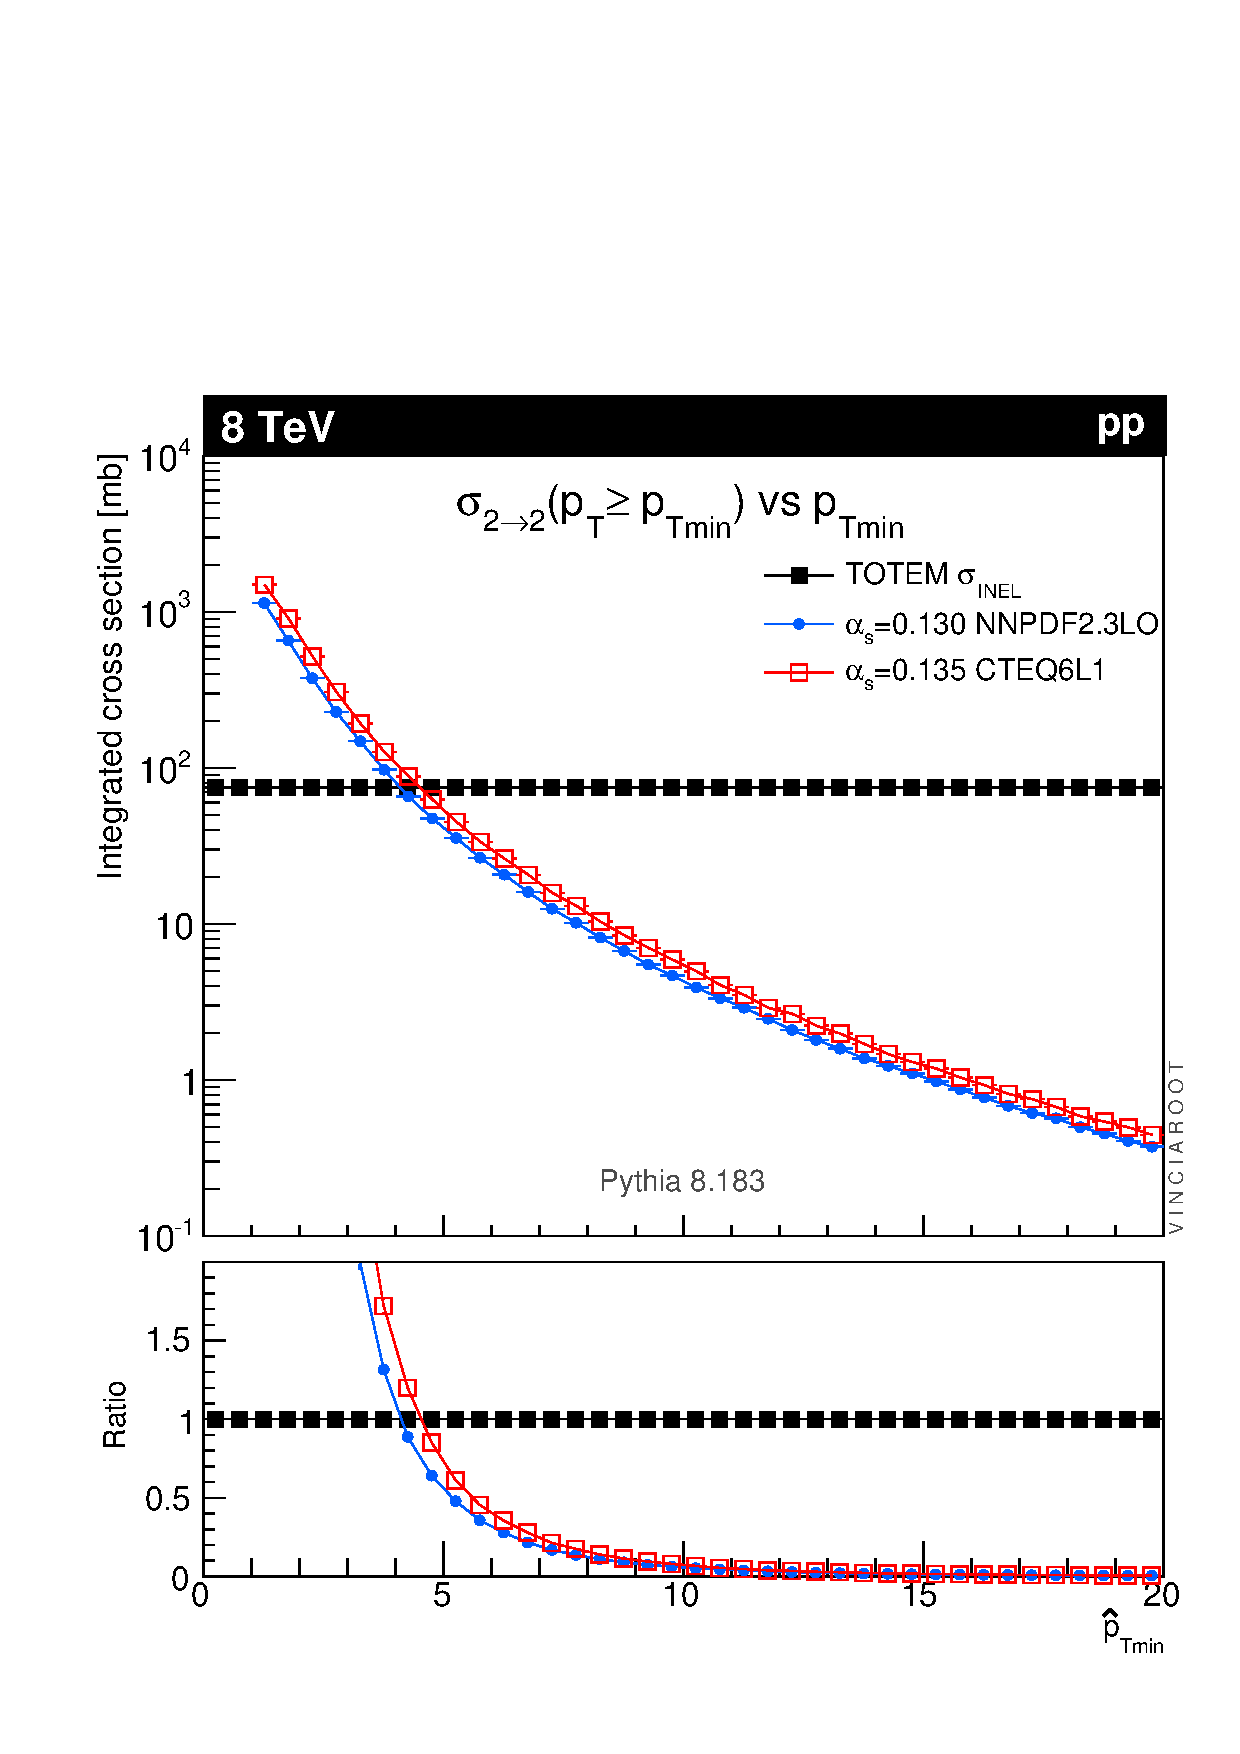
\includegraphics[scale=0.42]{sigma-8-sigma.pdf}
\caption{Proton-proton collisions at 8 TeV. LO QCD parton-parton
  cross section (integrated above 
  $p_{T\mrm{min}}$, for two different $\alpha_s$ and PDF choices)
  compared to the total inelastic hadron-hadron 
  cross section. Towards the right of the plot, we see, as
  expected, that hard dijet events is only a tiny fraction of the
  total cross section. The fact that the curves cross at a scale of
  order 5 GeV is interpreted to mean that this is a characteristic
  scale relevant for MPI. \cite{Skands:2014pea}.
\label{fig:sigmaQCD}
}
\end{figure}
In the context
of MPI models, this is interpreted straightforwardly 
to mean that \emph{each} hadron-hadron collision
contains \emph{several} few-GeV parton-parton collisions. 

In the limit that all the partonic interactions are independent and equivalent,
one would simply have a Poisson distribution in the number of MPI, with average
\begin{equation}
 \langle n \rangle(\ptmin{}) = \frac{\sigma_{2\to2}(\ptmin{})}
{\sigma_{\rm tot}} ~,
\end{equation}
with $\ptmin{}$ a lower cutoff scale which we shall return to below,
and $\sigma_\mrm{tot}$ a measure of the inelastic
hadron-hadron cross section. 
This simple reinterpretation in fact expresses unitarity;
instead of the total interaction cross
section diverging as $\ptmin{} \to 0$ (which would violate
unitarity), we have restated the problem so
that it is now the {\it number of MPI per collision} that
diverges, with the total cross section remaining finite. 

Two important ingredients remain to fully
regulate the remaining divergence. Firstly, the interactions cannot use up more
momentum than is available in the parent hadron. This 
 suppresses the large-$n$ tail of the estimate
above.
\index{PYTHIA}%
In \Py-based models, the
MPI are ordered in $\pt{}$~\cite{Sjostrand:1987su,Sjostrand:2004ef},
and the parton 
densities for each successive 
interaction are explicitly constructed so
that the sum of $x$ fractions can never be greater than unity. In
the \Hw\ models~\cite{Butterworth:1996zw,Bahr:2009ek}, instead the
uncorrelated estimate of  
$\langle n \rangle$ above is used as an initial guess, but
the generation of actual MPI is stopped once the
energy-momentum conservation limit is reached.

The second ingredient invoked to suppress the number of interactions,
at low $\pt{}$ and $x$, is colour screening; if 
the wavelength $\sim$ $1/\pt{}$ of an exchanged coloured parton 
becomes larger than a typical colour-anticolour separation distance, 
it will only see an {\it average} colour charge that vanishes in the limit
$\pt{} \to 0$, hence leading to suppressed interactions. 
This provides an infrared cutoff for
MPI similar to that provided by the hadronisation
scale for parton showers. 
A first estimate of the colour-screening cutoff would be 
the proton size, $
\ptmin{} \approx \hbar/r_{p} \approx
0.3~\mbox{GeV} \approx \Lambda_{\rm QCD}$, 
but empirically this appears to be far too low. In current models, one
replaces the proton radius $r_{p}$ in the above formula by a ``typical
colour screening distance,'' i.e.,\ an average size of a region within
which the net compensation of a given colour  
charge occurs. This number is not known from first 
principles, though it may be related to
saturation~\cite{Ryskin:2011qe}. In current MPI models, it is 
perceived of simply as an effective cutoff parameter, to be determined
from data. 

Note that  the partonic cross sections depend upon the PDF set used,
and therefore the optimal value to use for the 
cutoff will also depend on this
choice~\cite{Schulz:2011qy}. Note also that 
the cutoff does not have to be energy-independent. 
Higher energies imply that parton densities can be probed at smaller
$x$ values, where the number of partons rapidly increases. Partons
then become closer packed and the colour-screening distance $d$
decreases. The uncertainty on the scaling of the cutoff is a major concern when
extrapolating between different collider 
energies~\cite{Skands:2010ak,Schulz:2011qy,Skands:2013asa}. 

We now turn to the origin of the observational fact that hard jets appear to sit on top of a ``pedestal'' of underlying activity, which on average appears to be distributed evenly at all rapidities (i.e., also far from the jet cores). 
\begin{quote}
  ``Outside the [jet], a constant ET plateau is observed, whose height is independent of the jet ET. Its value is substantially higher than the one observed for minimum bias events.''~(\textbf{UA1} Collaboration (1983)~\cite{Arnison:1983gw})
\end{quote}
That is, the so-called ``underlying event'' (UE) is 
substantially more active, with larger fluctuations, than the average min-bias
event. In the MPI context, this is interpreted as a consequence of
impact-parameter-dependence: in peripheral
collisions, only a small fraction of events contain any
high-$\pt{}$ activity, whereas central collisions are more
likely to contain at least one hard scattering; a high-$\pt{}$ triggered
sample will therefore be biased towards small impact parameters, $b$,
with a larger number of MPI (and associated increased activity).

\begin{figure}[t]
  \centering
  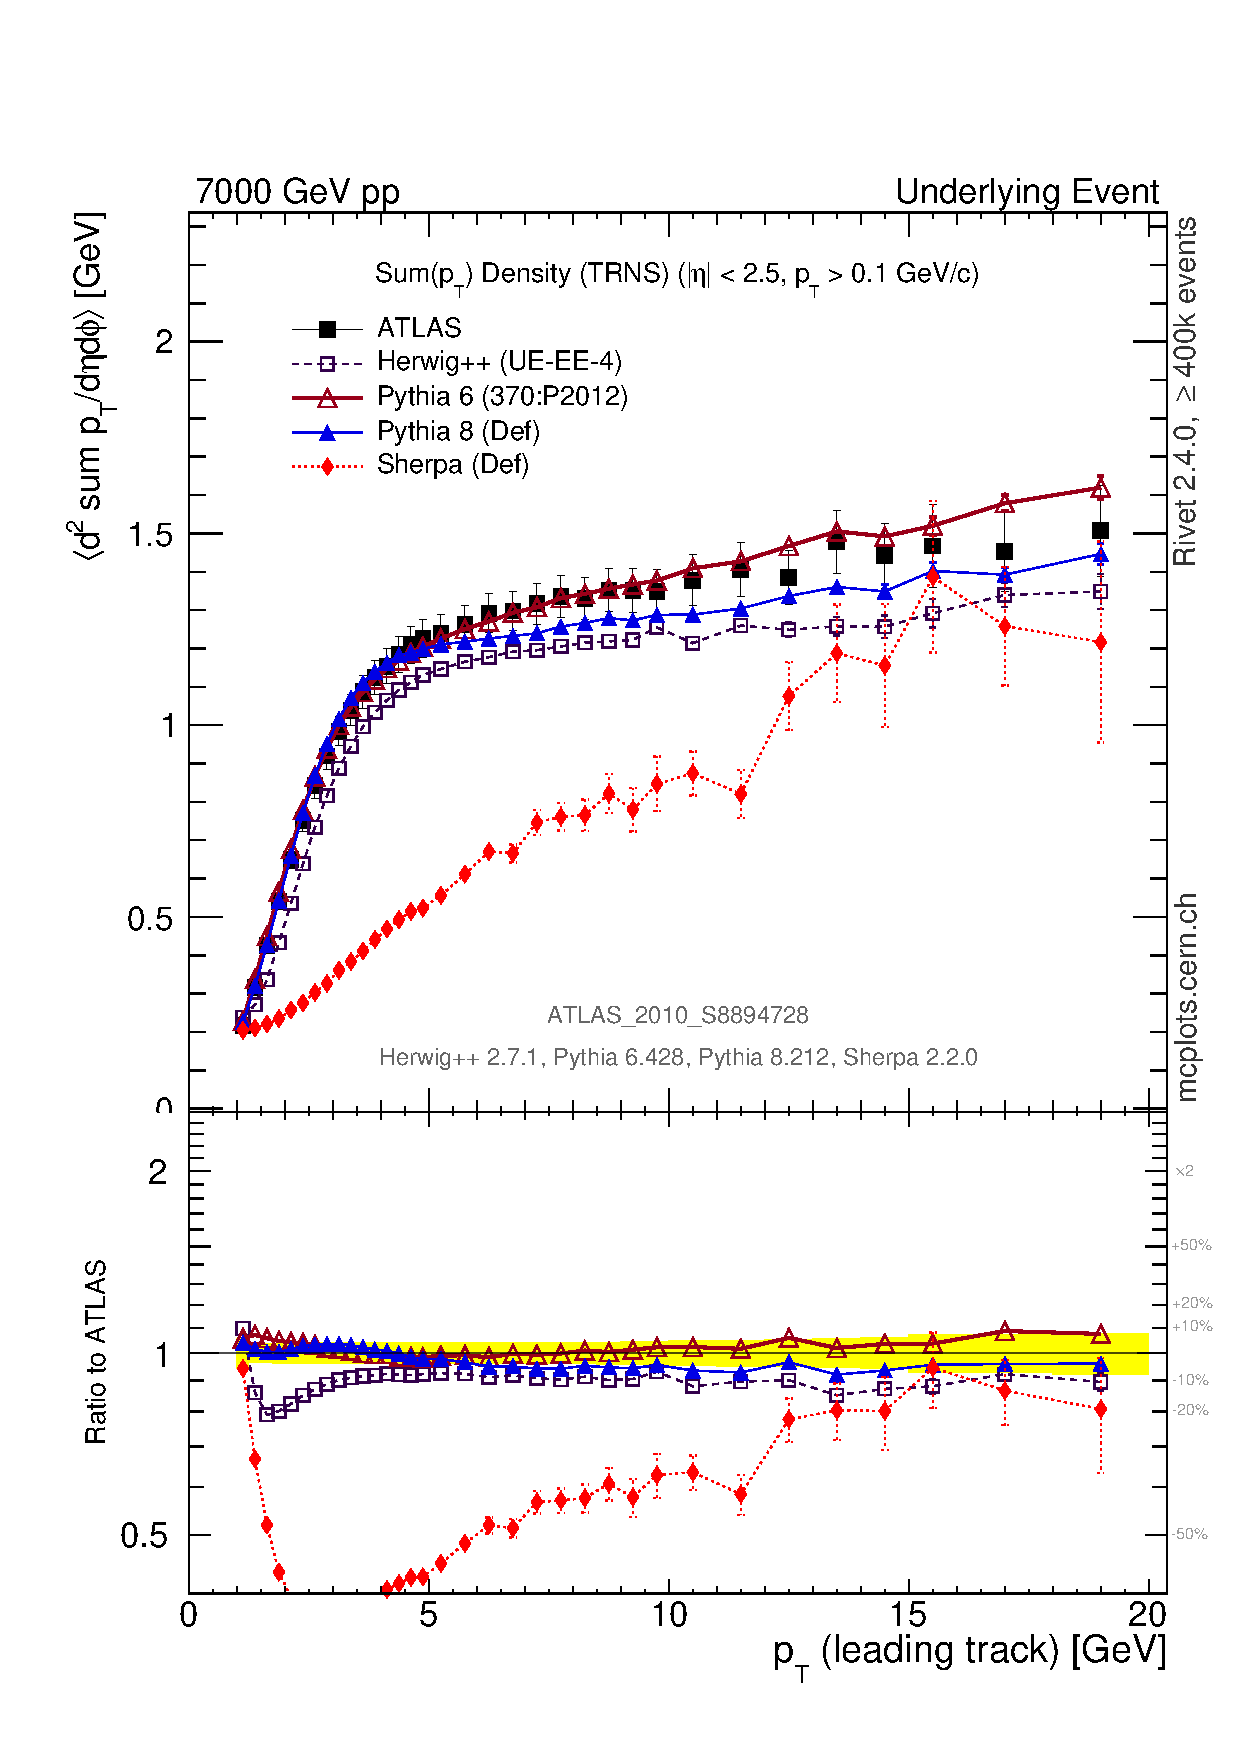
\includegraphics[scale=0.375]{uemb-hard-sumpt-vs-pt.pdf}~
  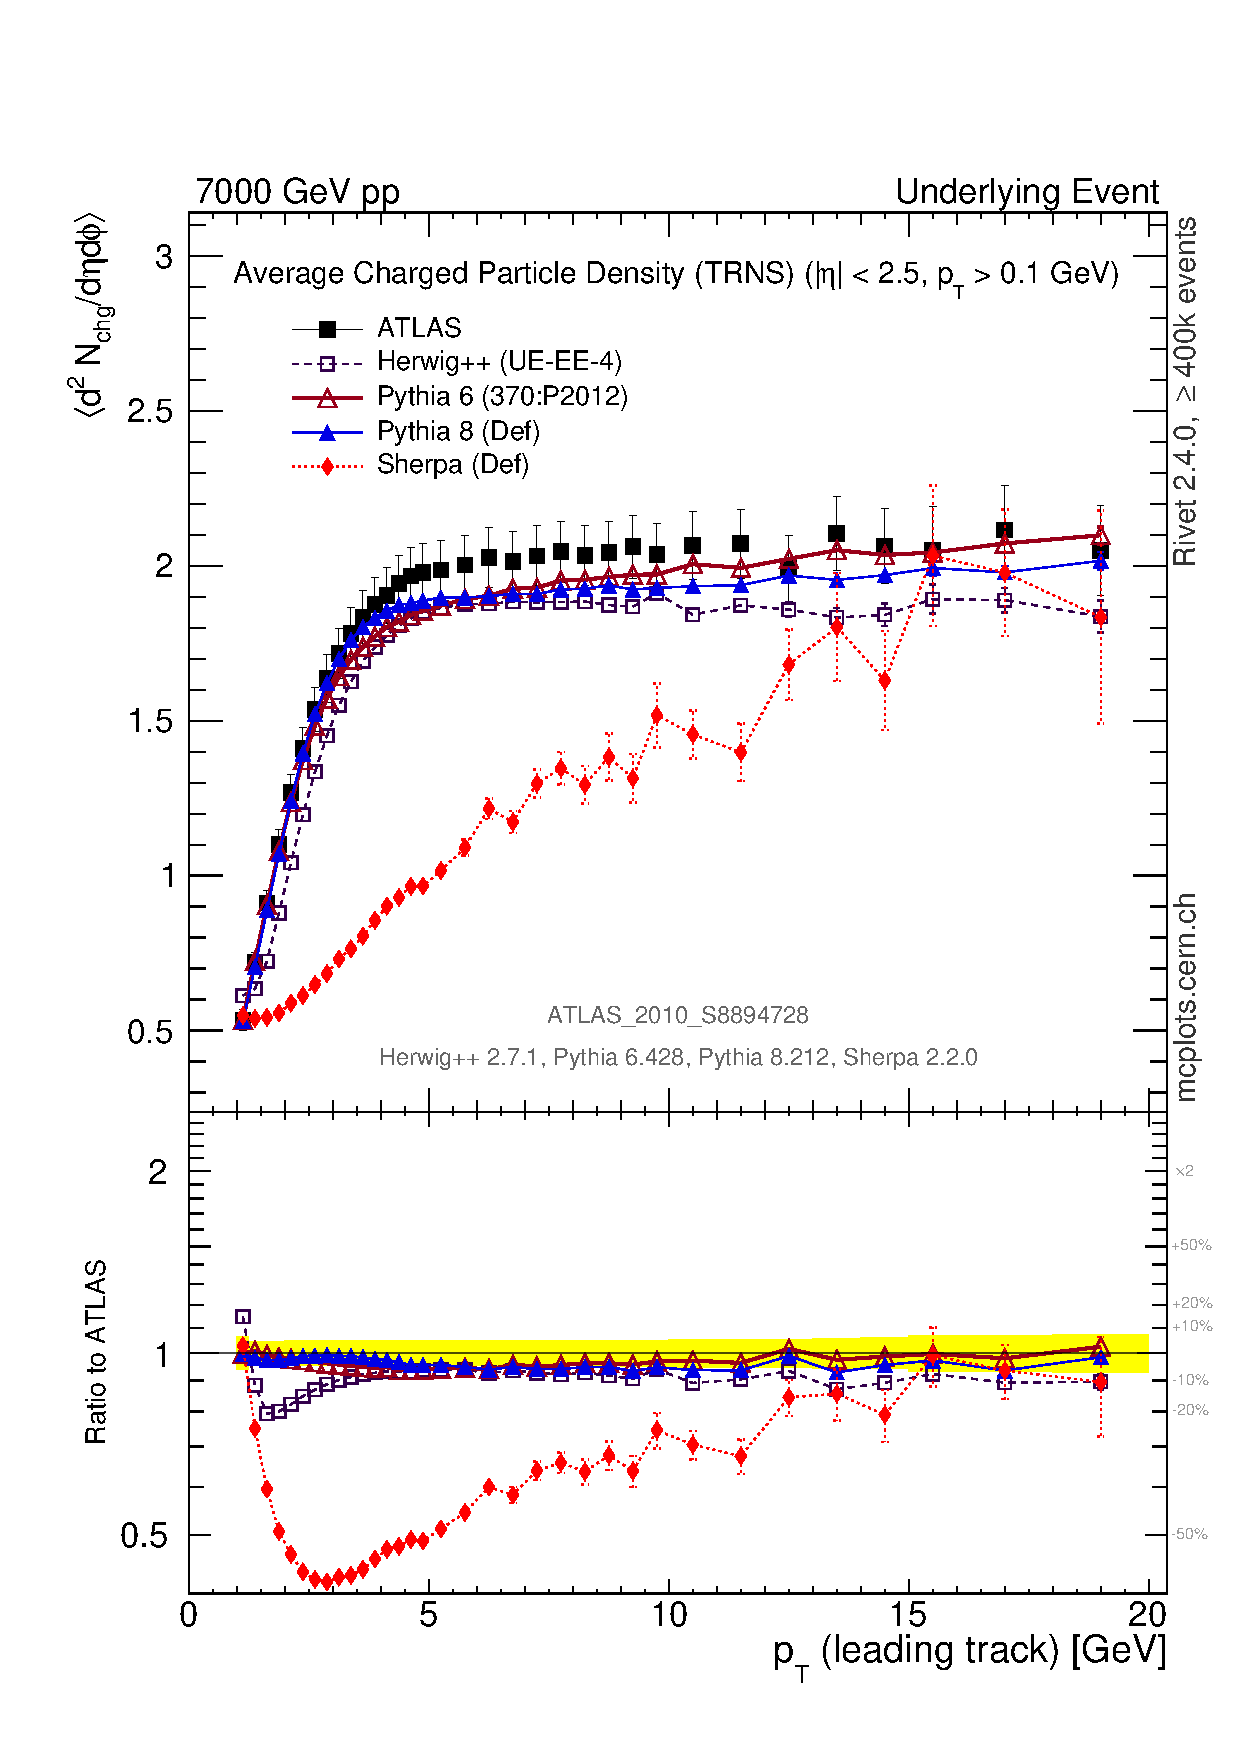
\includegraphics[scale=0.38]{uemb-hard-nch-vs-pt.pdf}
  \caption{The rise of the Underlying Event, as a function of leading-track $p_\perp$, as measured in the ``Transverse Region'' defined by azimuthal angles $60^\circ< \Delta\phi <120^\circ$ from the leading track, averaged over the available rapidity region. {\sl Left:}~average summed $p_\perp$ (per unit $\Delta\eta\Delta\phi$) for all tracks with $p_\perp>0.1$\,GeV. {\sl Right:}~average number of charged tracks (per unit $\Delta\eta\Delta\phi$) with $p_\perp>0.1$\,GeV. 
    Plots from  \href{http://mcplots.cern.ch}{mcplots.cern.ch}~\cite{Karneyeu:2013aha}.\label{fig:UElevel}}
\end{figure}
The rise of the pedestal level from low to high trigger-object\footnote{Different measurements and detectors employ different types of trigger objects, such as the leading track, leading track-jet, leading calorimeter jet, etc. In principle, the more inclusive (IR safe) the trigger is defined, the cleaner the measurement of the pedestal rise will be.} $p_\perp$ is illustrated in \figRef{fig:UElevel}. The leveling off of the distributions above leading-track $p_\perp$ values $\sim$ 5 GeV can be interpreted as an effect of ``maximum bias''; when the trigger $p_\perp$ is high enough, the selected events are essentially already maximally biased to small impact parameters, and from that point onwards the UE essentially becomes ``independent of the jet ET''~\cite{Arnison:1983gw} (modulo spillover of bremsstrahlung radiation from the hard-jet regions, which will still increase with the trigger-jet $p_\perp$; this component can be partially suppressed e.g.\ by vetoing events with bremsstrahlung; by considering only the least active of the two UE regions; or by systematically classifying all of the activity in the event as either ``jet-like'' or ``plateu-like''~\cite{Cacciari:2009dp}).
The ability of a theory model to describe the rise of the pedestal from the min-bias level to the UE plateau therefore depends upon its modeling of the $b$-dependence, and correspondingly the impact-parameter distribution (or, equivalently, the assumed mass distributions of the proton in $b$-space)
constitutes another main tuning parameter.   
\index{Monte Carlo!Tuning}%
A detailed discussion of impact-parameter dependent models goes beyond
the scope of these lectures;  
see \cite{Sjostrand:1987su,Sjostrand:2004pf,oai:arXiv.org:1101.5953}.  

For hard processes at the LHC at 13 TeV, the transverse energy, $E_T$, in the
UE is expected to be about $3.3~\mbox{GeV}$ per unit $\Delta
R=\sqrt{\Delta\phi^2+\Delta\eta^2}$ 
area~\cite{Skands:2013asa} (for a reference case of 100-GeV dijets, 
including both charged and neutral particles, with no cut on $p_\perp$), 
though with large event-to-event fluctuations of order $\pm
2~\mbox{GeV}$~\cite{Aad:2010fh}. Thus, for example, the total $E_T$
originating from the UE,  
in a cone with radius $0.4$ can be estimated to
be $E_{T\mrm{UE}}(R=0.4)\sim 1.6\pm 1~\mbox{GeV}$, 
while the $E_T$ in a cone with radius $1.0$ would be
$E_{T\mrm{UE}}(R=1.0)\sim 10\pm 6~\mbox{GeV}$. Note that the magnetic
field in realistic detectors will deflect some fraction of the soft charged
component of the underlying event into helix trajectories that will
hence not contribute to the energy deposition in the
calorimeters. 

\subsection{Tuning \label{sec:tuning}} 
\index{Tuning|see{Monte Carlo}}%
\index{Monte Carlo!Tuning}%
\index{Monte Carlo!Event generators}%
\index{Monte Carlo!Uncertainties}%

A main virtue of general-purpose Monte Carlo event generators
is their ability to
provide a complete and fully differential picture of collider final
states, down to the level of individual particles. 
As has been emphasised in these lectures, 
the achievable accuracy depends both on the
inclusiveness of the chosen observable and on the  
sophistication of the simulation itself. An important driver for the
latter is obviously the development of improved theoretical models,
e.g., by including matching to higher-order matrix elements, more
accurate resummations, or better non-perturbative models,  as
discussed in the previous sections; but it  
also depends crucially on the available constraints on the remaining
free parameters of the model. Using existing data (or more precise
calculations) to constrain these is referred to as generator
tuning. 

Keep in mind that generators attempt to deliver a \emph{global}
description of the data; a tune is no good if it fits one distribution
perfectly, but not any others. It is therefore crucial to study the
simultaneous degree of agreement or disagreement over many, mutually
complementary, distributions. 
A useful online resource for making such comparisons can be found at
the \href{http://mcplots.cern.ch}{MCPLOTS} web
site\cite{Karneyeu:2013aha} (which relies on computing power donated
by volunteers,
via the \href{http://lhcathome.web.cern.ch/test4theory}{LHC@home} project~\cite{Lombra?aGonz?lez:2012zz}). The
analyses come from the comprehensive \textsc{Rivet} analysis
toolkit~\cite{Buckley:2010ar}, which can also be run stand-alone to
make your own MC tests and comparisons.

\index{Monte Carlo!Event generators}%
Although MC models may appear to have a
bewildering number of independently adjustable parameters, 
it is worth noting that most  of these only control
relatively small (exclusive) details of the event generation. The
majority of the 
(inclusive) physics is determined by only a few, very important ones, 
such as the value of the strong coupling, in the perturbative
domain, and the form of the fragmentation function for massless
partons, in the non-perturbative one. 

Armed with a good understanding of the underlying model, an expert would
therefore normally take a highly factorised approach to constraining
the parameters, 
first constraining the perturbative ones (using IR safe observables
and/or more precise theory calculations) and thereafter the
non-perturbative ones, each ordered in a measure of their relative
significance to the overall modeling. This  allows one 
to concentrate on just a few parameters and a few carefully chosen 
distributions at a time, reducing the full parameter space to manageable-sized
chunks. Still, each step will often involve more than one single
parameter, and non-factorisable 
correlations may still necessitate additional iterations from
the beginning before a fully satisfactory set of parameters is obtained. 

Recent years have seen the emergence
of automated tools that attempt to reduce the amount of both computer
and manpower required for this task, for instance 
by making full generator runs only for a
limited set of parameter points, and then interpolating between
these  to obtain approximations to what the true generator result
would have been for any intermediate parameter point, as, e.g., in 
\textsc{Professor}~\cite{Buckley:2009bj}. 
Automating the human expert input is more difficult. 
Currently, this is addressed by a combination of input solicited from
the generator authors (e.g., which parameters and ranges to consider,
which observables constitute a complete set, etc)
and the elaborate construction of non-trivial weighting
functions that determine how much weight is assigned to each 
individual bin in each distribution. The field is still
burgeoning, and future sophistications are to be
expected. 
Nevertheless, at this point the overall quality of the tunes
obtained with automated methods appear to at least be competitive with
the manual ones. 

\index{Monte Carlo!Event generators}%
However, though we have very good LHC tunes for essentially all the
general-purpose generators by now, there are two important aspects
which have so far been neglected, and which it is becoming
increasingly urgent to address. The first is that a central tune is
not really worth much, unless you know what the uncertainty on it is. 
A few individual proposals for systematic tuning variations have
been made~\cite{Skands:2010ak,Richardson:2012bn}, but so far there is
no general approach for 
establishing MC uncertainties by tune variations. 
(Note: in 2016 all of the general-purpose MC collaborations
published strategies for automated evaluations of
perturbative shower uncertainties, which we highly recommend the
community to start using, see~\cite{Badger:2016bpw,Mrenna:2016sih,Bellm:2016voq}.)
The second issue is
that virtually all generator tuning is done at the ``pure'' LL shower
level,  and not much is known about what happens
to the tuning when matrix-element matching is subsequently
included\footnote{One aspect, consistent $\alpha_s$ variations, is
  discussed in ~\cite{Cooper:2011gk}.}.

Finally, rather than performing one global tune to all the
data, as is usually done,  a more systematic check on the validity of
the underlying physics model could be obtained by instead performing
several independent 
optimisations of the model parameters for a range of different 
phase-space windows and/or collider environments.
In regions in which consistent parameter sets are obtained (with
reasonable $\Delta\chi^2$ values), 
the underlying 
model can be considered as interpolating well, i.e., it is universal. 
If not, a breakdown in the ability of the model to span different
physical regimes has been identified, and can be addressed, with the
nature of the deviations giving clues as to the nature of the breakdown. 
With the advent of automated tools,  
such systematic studies are now becoming feasible, with a first
example given in \cite{Schulz:2011qy}. 

\index{Monte Carlo!Event generators}%
\index{Monte Carlo!Tuning}%
We round off by giving a sketch of a reasonably complete tuning
procedure, without going into details about the parameters that
control each of these sectors in individual Monte Carlo models 
(a recent detailed discussion in the context of PYTHIA 8 can be found
in~\cite{Skands:2014pea}): 

{\bf 1) Keep in mind} that inabilities of models to
 describe data is a vital part of the feedback cycle between
 theory and experiment. Also keep in mind that
 perturbation theory at (N)LO+LL is doing \emph{very well} if it gets
 within 10\% of a given IR safe measurement. An agreement of 5\% should be
 considered the absolute sanity limit, beyond which it does not make
 any sense to tune further. For some quantities, e.g., ones for which
 the underlying modeling is \emph{known} to be poor, an order-of-magnitude
  agreement or worse may have to be accepted. 
 
\index{String model}%
\textbf{2) Final-State Radiation and Hadronisation:} 
 mainly using LEP and other $e^+e^-$ collider data. On the IR safe
 side, there are event shapes and jet observables. On the IR sensitive
 side, multiplicities and particle spectra. Pay attention to 
 the high-$z$ tail of the fragmentation,
 where a single hadron carries a large fraction of an entire jet's
 momentum (most likely to give ``fakes''). 
Depending on the focus of the tuning, attention should also
 be paid to identified-particle rates and ratios (perhaps with a nod
 to hadron-collider measurements), and to fragmentation
 in events containing heavy quarks and/or gluon jets. 
 Usually, more weight is given to
 those particles that are most copiously produced. The scaling
 properties of IR safe vs.\ IR sensitive contributions can be
 tested by comparing data at several different $e^+e^-$ collider
 energies.  
 
\textbf{3) Initial-State Radiation, and 
  ``Primordial\footnote{Primordial $k_T$: an
  additional soft \pt\ component that is injected on top of the
  \pt\ generated by the initial-state shower itself, see
  \cite[Section 7.1]{Buckley:2011ms}.} $k_T$'':} the main constraining
  distribution is the dilepton \pt\ distribution in Drell-Yan events in
  hadron-hadron collisions. Ideally, one would like to use 
  several different $Q^2$ values, and/or complementary processes,
  like $p_\perp(\mrm{dijet})$ or $p_\perp(t\bar{t})$. 
For any observables containing explicit
  jets, be aware that the UE can produce small 
  horisontal shifts in jet \pt\ distributions, which may in turn 
  result in larger-than-expected 
  vertical changes if the distributions are falling sharply. Also note
  that the ISR evolution is sensitive to the choice of PDFs.

\textbf{4) Initial-Final Connections:} (radiation from
  colour lines connecting the initial and final states): 
\index{DIS}%
DIS and jet broadening in hadron collisions. This is one of the
  most poorly controlled parts of most MC models, highly sensitive to
  the treatment of coherence (see e.g.~\cite{Ritzmann:2012ca} for
  illustrations).  
  Keep in mind that it
  is \emph{not} directly constrained by pure final-state observables,
  such as LEP fragmentation, nor by pure initial-state observables,
  such as the Drell-Yan \pt\ spectrum, which is why we list it as a
  separate item here. The modeling of this
  aspect can have important effects on specific observables, a recent
  example being the $t\bar{t}$ forward-backward asymmetry at the
  Tevatron~\cite{Skands:2012mm}.

\textbf{5) Underlying Event:} Good constraints on the overall level of the
  underlying event can be obtained by counting the summed transverse
  energy (more IR safe) and/or particle multiplicities and average
  transverse momenta (more IR sensitive) in regions \emph{transverse}
  to a hard trigger jet (more IR safe) or particle (more IR
  sensitive), see e.g.~\cite{Field:2011iq}. 
  Constraints on the \emph{fluctuations} of the underlying
  event are also important, and can be obtained, e.g., by comparing to
  measurements of the RMS of such distributions~\cite{Aad:2010fh} or
  by plotting salient quantities along an axis from low to high UE
  activity~\cite{Martin:2016igp}. Again, note
  that the UE modelling can be very sensitive to the choice of
  PDFs~\cite{Schulz:2011qy,Skands:2014pea}. Finally, the modeling of
  the UE should be \emph{universal}, hence the same UE model should
  --- ideally --- be able to describe UE distributions not only in
  inclusive-jet events, but also the UE in processes like
  Drell-Yan~\cite{Aaltonen:2010rm,Chatrchyan:2012tb,Aad:2014jgf,Alioli:2016wqt}
  or  $t\bar{t}$ production~\cite{CMS:2013mfa,CMS:2015usp}.  

\index{String model}%
\index{Colour connections}%
\textbf{6) Colour (Re-)Connections and other Final-State Interactions:}  
 By Final-State Interactions,
  we intend a broad spectrum of possible collective effects that may
  be included to a greater or lesser extent in various models. These
  effects include: Bose-Einstein correlations (see,
  e.g., \cite{Lonnblad:1997kk}), 
rescattering (see, e.g., \cite{Corke:2009tk}), 
colour reconnections / string
  interactions  (see,
  e.g., \cite{Rathsman:1998tp,Skands:2007zg,Bopp:2011fw,Gieseke:2012ft,Christiansen:2015yqa}),  
  hydrodynamics (see, e.g., \cite{Werner:2011zzc}), 
etc. 
  As a rule, these effects
  are soft and/or non-perturbative and hence should not modify hard IR safe
  observables appreciably. They can, 
  however, have \emph{drastic} effects on IR sensitive ones, such as
  particle multiplicities, momentum distributions, and correlations, 
  wherefore useful constraints are typically furnished by 
  measurements of spectra and correlations as functions of
  quantities believed to 
  serve as indicators of the strength of these phenomena 
  (such as event multiplicity~\cite{Petrov:2012hca,Bierlich:2015rha,Adam:2016emw} or underlying-event
  activity~\cite{Martin:2016igp}), and/or by collective-flow-type 
  measurements. 
  Finally, if the model includes a universal description of
  underlying-event and soft-inclusive QCD, as many MPI-based models do, then
  minimum-bias data can also be used as a control sample, though one must
  then be careful either to address diffractive contributions properly
  or to include only gap-suppressed data samples. A complete MB and UE
  model should also be able to describe the rise of the pedestal from
  MB to UE, e.g., in the transverse UE observables (see above).

\textbf{7) Beam Remnants:} Constraints on beam-remnant fragmentation
(see, e.g., \cite{Sjostrand:2004pf}) are most directly obtained in the forward
  region~\cite{Chatrchyan:2011wm,Chatrchyan:2011wb,Aspell:2012ux,Chatrchyan:2013gfi,Aaij:2014pza,Chatrchyan:2014qka,Antchev:2014lez}. Especially
  for soft-inclusive triggers, cuts designed to isolate diffractive
  topologies are then required to distinguish effectively between the
  fragmentation of a (diffractive) colour-singlet excitation of the
  beam particle and that of a (non-diffractive) colour-charged
  remnant having exchanged some (non-zero) net amount of
  colour charge with the other colliding beam hadron. To lowest
  order, the remnant should be in a triplet (octet) colour state after
  having exchanged a quark (gluon) with the other beam particle, but
  taking MPI into account much larger amounts of colour may be
  transferred, with correspondingly larger possible colour
  representations of the remnant (see, e.g.,~\cite{Christiansen:2015yqa}). 
The amount of baryon transport from the remnant
  to a given rapidity region~\cite{Erhan:1979ba,Aaij:2011va,Abazov:2015sri} can
  also be used to probe how much the colour 
  structure of the remnant was effectively disturbed, with more baryon
  transport indicating a larger amount of ``beam baryon blowup''.
Ideally one would also correlate the forward activity with a (central) measure of
how much total colour charge is scattered out of the remnant(s), such as
an observable sensitive to the number of MPI. 
